
\chapter{Introduction}

\section{About company}
 Node robotics GmbH is the spin-off of Fraunhofer Institute for Manufacturing Engineering and Automation IPA, Stuttgart. In 2013 NODE software technology development stated in Fraunhofer IPA. Later in 2015 NODE software has been implemented on 30 AMR's in Audi & Bär Automation. In 2018 project with BMW started for the largest automation project. In March 2020, Node receives funding from German Federal Ministry for Economic Affairs and Energy(BMWi). With this NODE Robotics GmbH founded in November 2020. In December 2020, successful investments completed by pre-seed investors.
\begin{figure}[h]
	\begin{center}
		
\includegraphics[height=2.5cm]{images/download.png}
		\caption{NODE Robotics GmbH}
	\end{center}
\end{figure}
 
 Node robotics offers plug\&play software solutions for autonomous intralogistics. The main focus of the company is to bring in multiple robots to co-ordinate each other in path planning. Thus enabling the driver-less transport vehicles and AGV's to autonomous mobile robots. Thus the software solution provided by the company mainly focuses on providing autonomous and collaborative fleets which helps the multiple robots to communicate and support each other. In doing so NODE provides the basis for the widespread use of autonomous mobile robots(AMR) in production and intralogistics[1].
 The three main component which makes NODE solution better are
 \begin{enumerate}
 	\item Live SLAM:
 	
 	The Live SLAM realizes this through probabilistic localization methods in combination with continuous map updating. In the basic setup, the sensor data of the 2D (safety) LIDAR sensors are sufficient for this. Optionally, further sensor systems such as 3D LIDAR, camera systems, GPS/UWB, etc. can be integrated. In addition to localization, Live SLAM provides the current map of the environment as a basis for e.g. dynamic route planning and traffic management. 
 	\item Online Route Planning:
 	
 	Calculate the best route at runtime even in large, variable industrial environments? The online route planner calculates the optimal route between any start/destination at runtime based on the current map and user-defined traffic zones (such as one-way streets, no-go zones, etc.). The route calculation takes into account robot-specific properties such as kinematics, dimensions including speed-dependent safety fields and loading condition.
 	
 	\item Dynamic Motion Planning:
 	
 	 Dynamic motion planning ensures efficient execution of the global route and collision avoidance by calculating optimal trajectories and speed commands. It takes into account both internal constraints of the AMR (kinematics, dynamics, footprint, safety fields) and obstacles detected in real time with onboard sensor technology (2D/3D LIDAR, camera systems).
 \end{enumerate}

 Main vision of NODE is to enable any type of mobile robot to be universally deployed on any factory floor as an autonomous means od transport. While the mission of NODE is to provide a software solution through targeted research, development and quality focus that enables any company to bring its intralogistics into the age of Industry 4.0 through fast commissioning and intuitive usability.
 
 With NODE.OS, Node offers a holistic software solution-from order management to AMR control- co-ordinative path planning- versatile in use according to the requirements. 
 
 The solutions provided by NODE includes: 
 \begin{enumerate}
 	\item Industrial-proof: All the solutions are developed and tested in an industrial environment
 	\item One software fits all: Modular approach independent of hardware. NODE also provides choice of more than 10 software modules that can be used independently of each other.
 	\item Future-proof: All the developments are based on the latest approaches in the field of ROS, cloud robotics and machine learning
 \end{enumerate}
 
 With NODE software about 450 AMR's and 27 different AMR types are in productive use in different warehouses and manufacturing areas of different customers. Some of the AMR's includes MIR, different versions of BMW-STR, Care-O-Bot etc.      
 
 

\section{Modular approach}
As discussed above NODE provides the modular approach. NODE Robotics aims to provide the Autonomous navigation and fleet management as one solution. Autonomous navigation includes the part of path-planning between start point and destination. This also includes obstacle avoidance both dynamically and statically. 
\begin{figure}[h]
	\begin{center}
		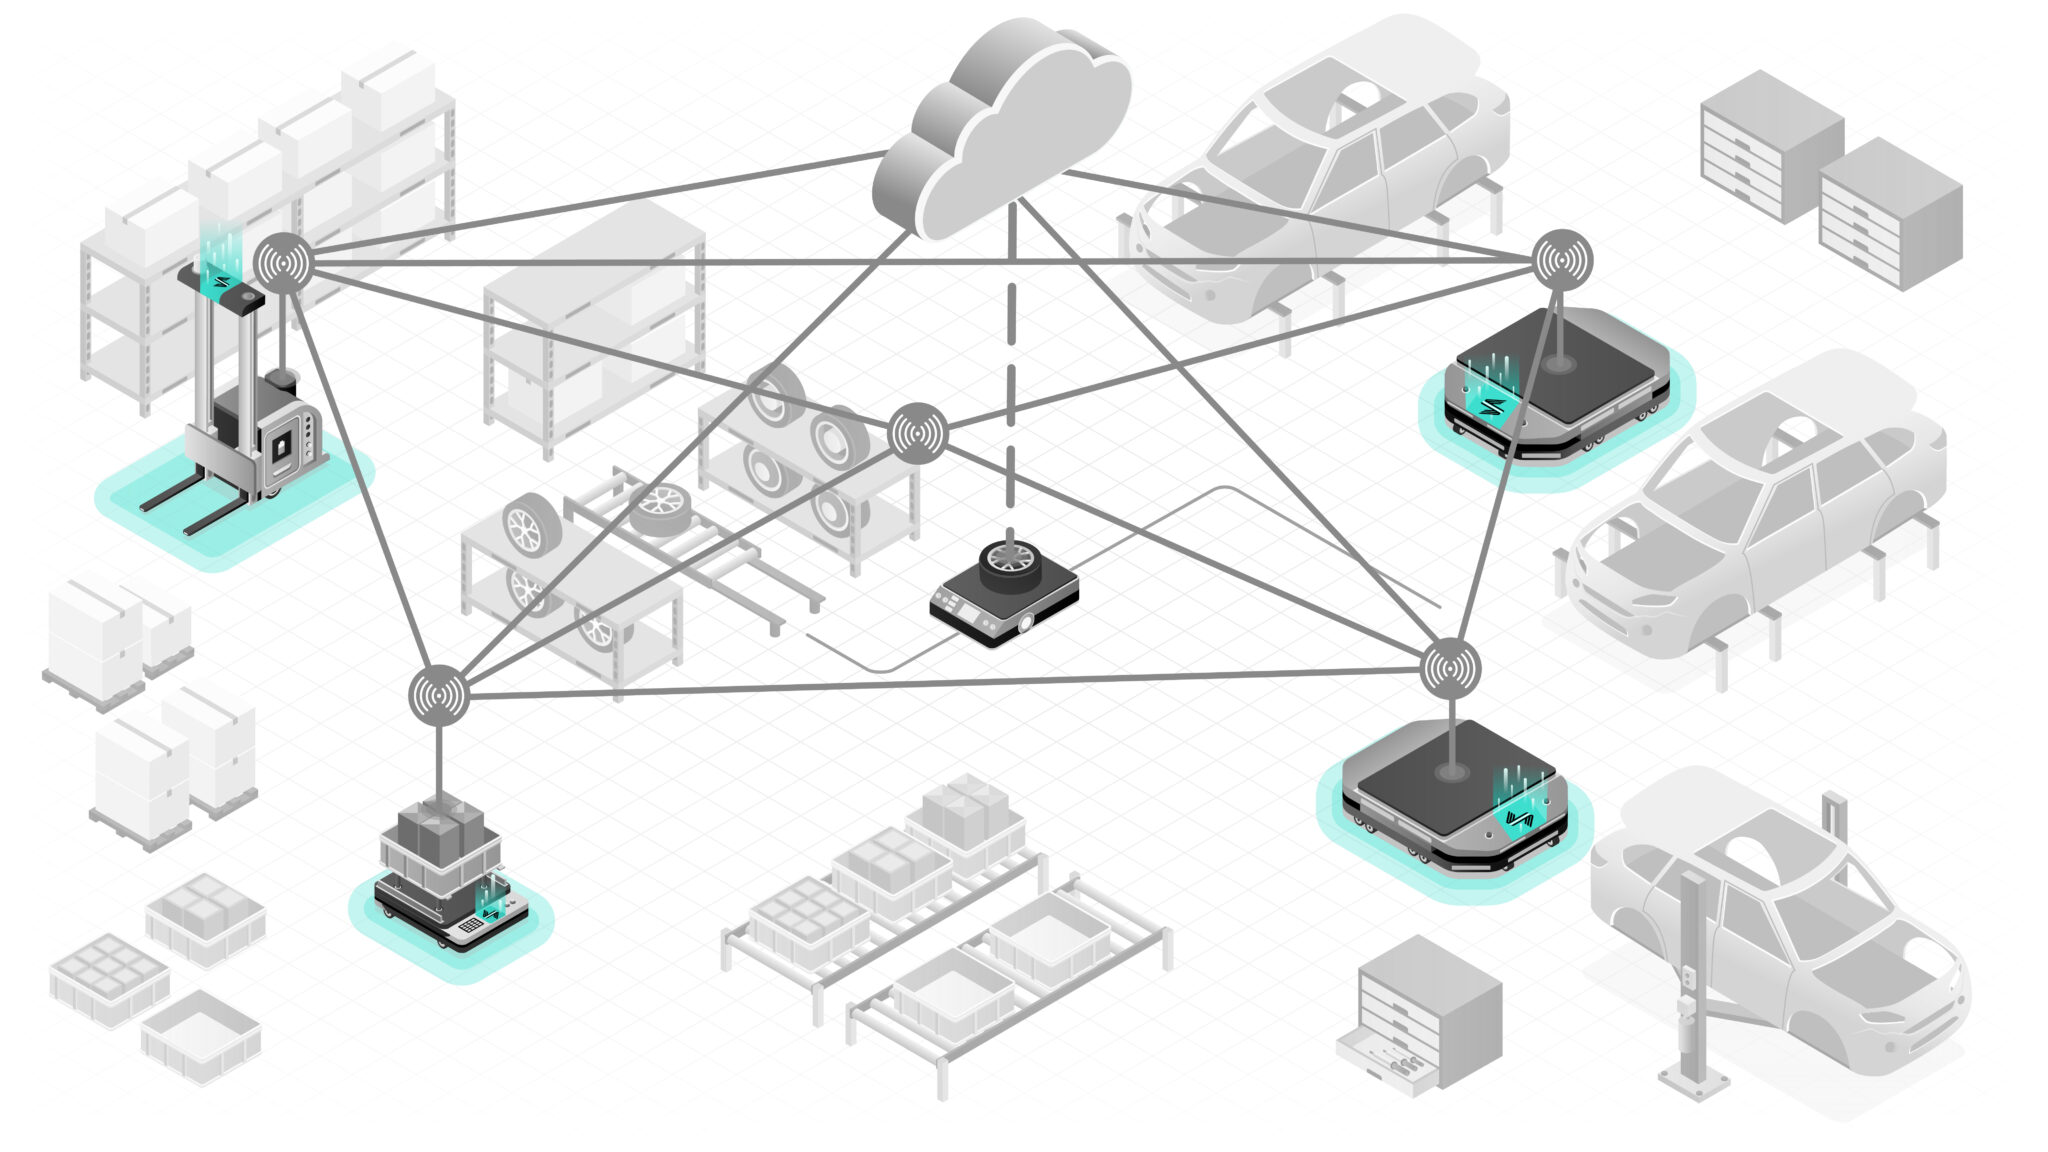
\includegraphics[height=9 cm]{images/structure.jpg}
		\caption{Basic capability of AMR for autonomous navigation}
	\end{center}
\end{figure}

Fleet management includes the inter-communication between robots and collaboration in path planning for multiple robots. 

To achieve both Autonomous navigation and fleet management with modularity, NODE provides four different components which are as listed
\begin{enumerate}
	\item NODE.OS
	\item NODE.EDGE
	\item NODE.MESH
	\item NODE.SRVS
\end{enumerate}

\subsection{NODE.OS}
NODE.OS is based on three independent but aligned software modules.
\subsection{NODE.EDGE}
NODE.EDGE is the software component which runs at the robot level. This software is used by the individual AMR to plan the path and navigate itself to the desired destination. This also includes the static obstacle avoidance. Continuously updated environment and data models enable the NODE.EDGE to adapt to environmental changes in real time and to cope with unforeseen situations. If desired, the AMRs avoid obstacles such as other vehicles or people and successfully execute even previously unknown orders.
\subsection{NODE.MESH}
NODE.MESH is the software component which helps for the collaboration of multiple AMR's. This includes obstacle avoidance dynamically and communicating between the robots will also ensures the shortest path without obstacles.
image here

\begin{figure}[h]
	\begin{center}
		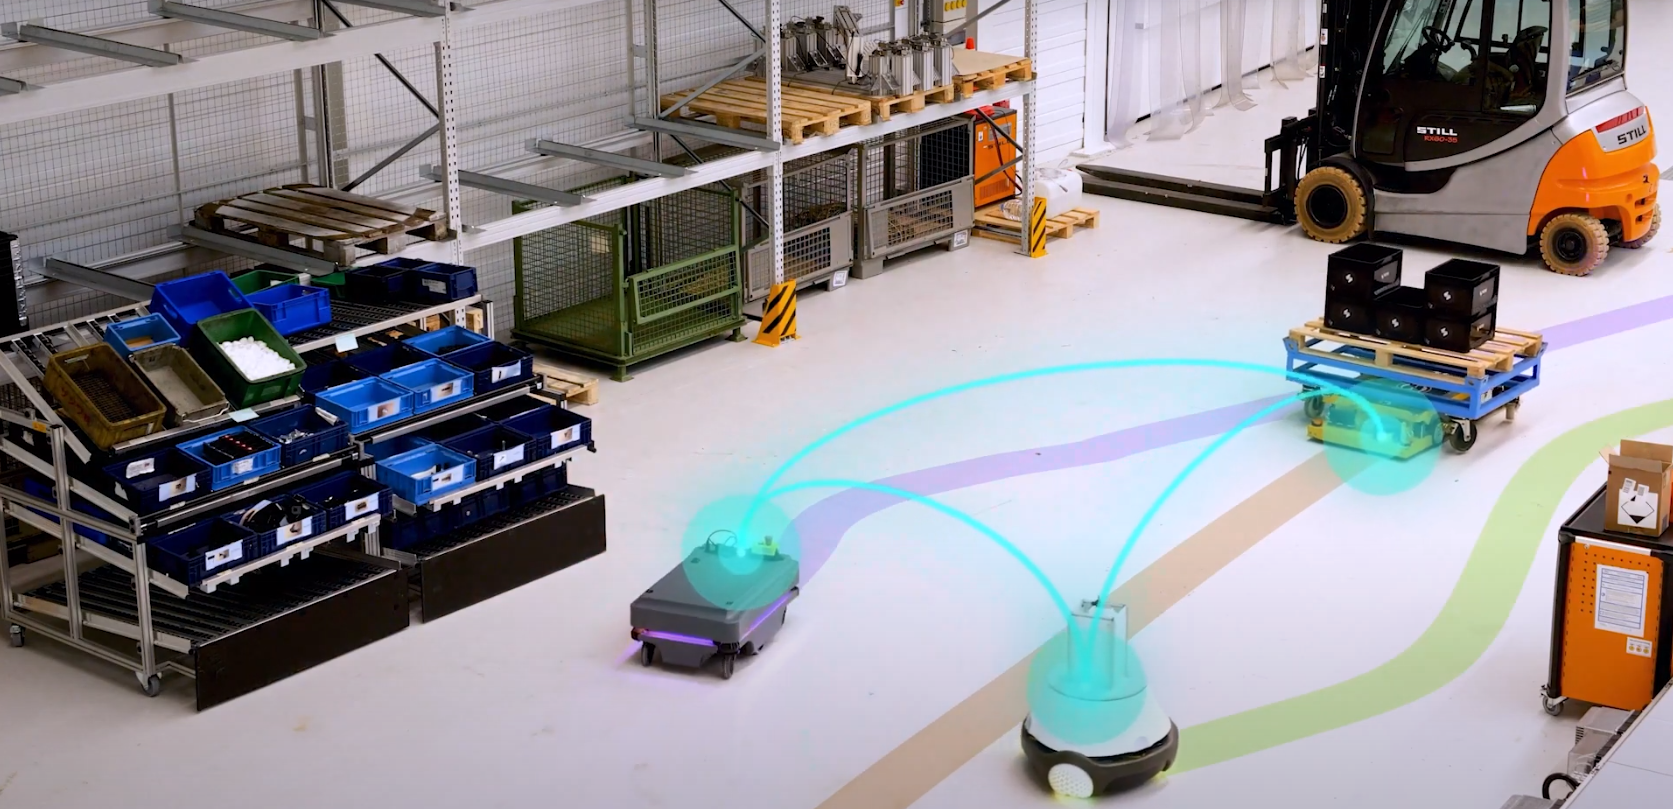
\includegraphics[height=5cm]{images/mesh.png}
		\caption{Collaboration of robots}
	\end{center}
\end{figure}
\subsection{NODE.SRVS}
NODE.SRVS will deals with cloud level fleet management and coordination of robots.

\vspace{0.5cm}
As an interface the VDA5050 standards are used along with Open API, to realize the autonomous fleets

\pagebreak
\section{Different teams of the company}
NODE Robotics has four different teams
\begin{enumerate}
	\item Perception and SLAM
	\item Fleet management system(FMS)
	\item Operations
	\item UI/UX

\end{enumerate}
\subsection{Perception and SLAM}
 This teams works with the mapping of the surrounding environment. Simultaneous localization and mapping will help the robot to localize itself inside the map. This part will also take care of creating the map from the LIDAR scanners. Basically main aim is to achieve the fastest localization of the robot in the current environment with matching the scans and obstacles present in the map. Also this team aims at creating the dynamic map based on inputs provided from the multiple robots.

\subsection{Fleet management system(FMS)}
Fleet management team works basically with the traffic management of the multiple robots. This team works with planned execution of mission and managing fleets. The Fleet Management System is a software package for transport mission of AGV's. On the plant operation side, this is achieved by exposing a unified REST-API for submitting POI's and also zones for traffic management.
\subsection{Operations}
Operations team work as bridge between the implementation of the algorithm and executing on the robot. This team also try to implement the backend like FMS stuff all on docker, so that implementation is easy and can be implemented everywhere without any implementation restriction. Also helps as the backend support for the frontend UI/UX department.
\subsection{UI/UX}
This team helps in visualizing the robots and map on the own frontend side. This helps in visualizing the robots, path and dedicated zones for the robots. This team is also trying to do the 3D representation of the robots and environment of the working area.

The following image in Figure 1.4 shows the appearance of NODE own frontend tool along with the robots and there path. In this same picture we can see some point names like south\_corner2 which indicates the point of interest. 

\begin{figure}[h]
	\begin{center}
		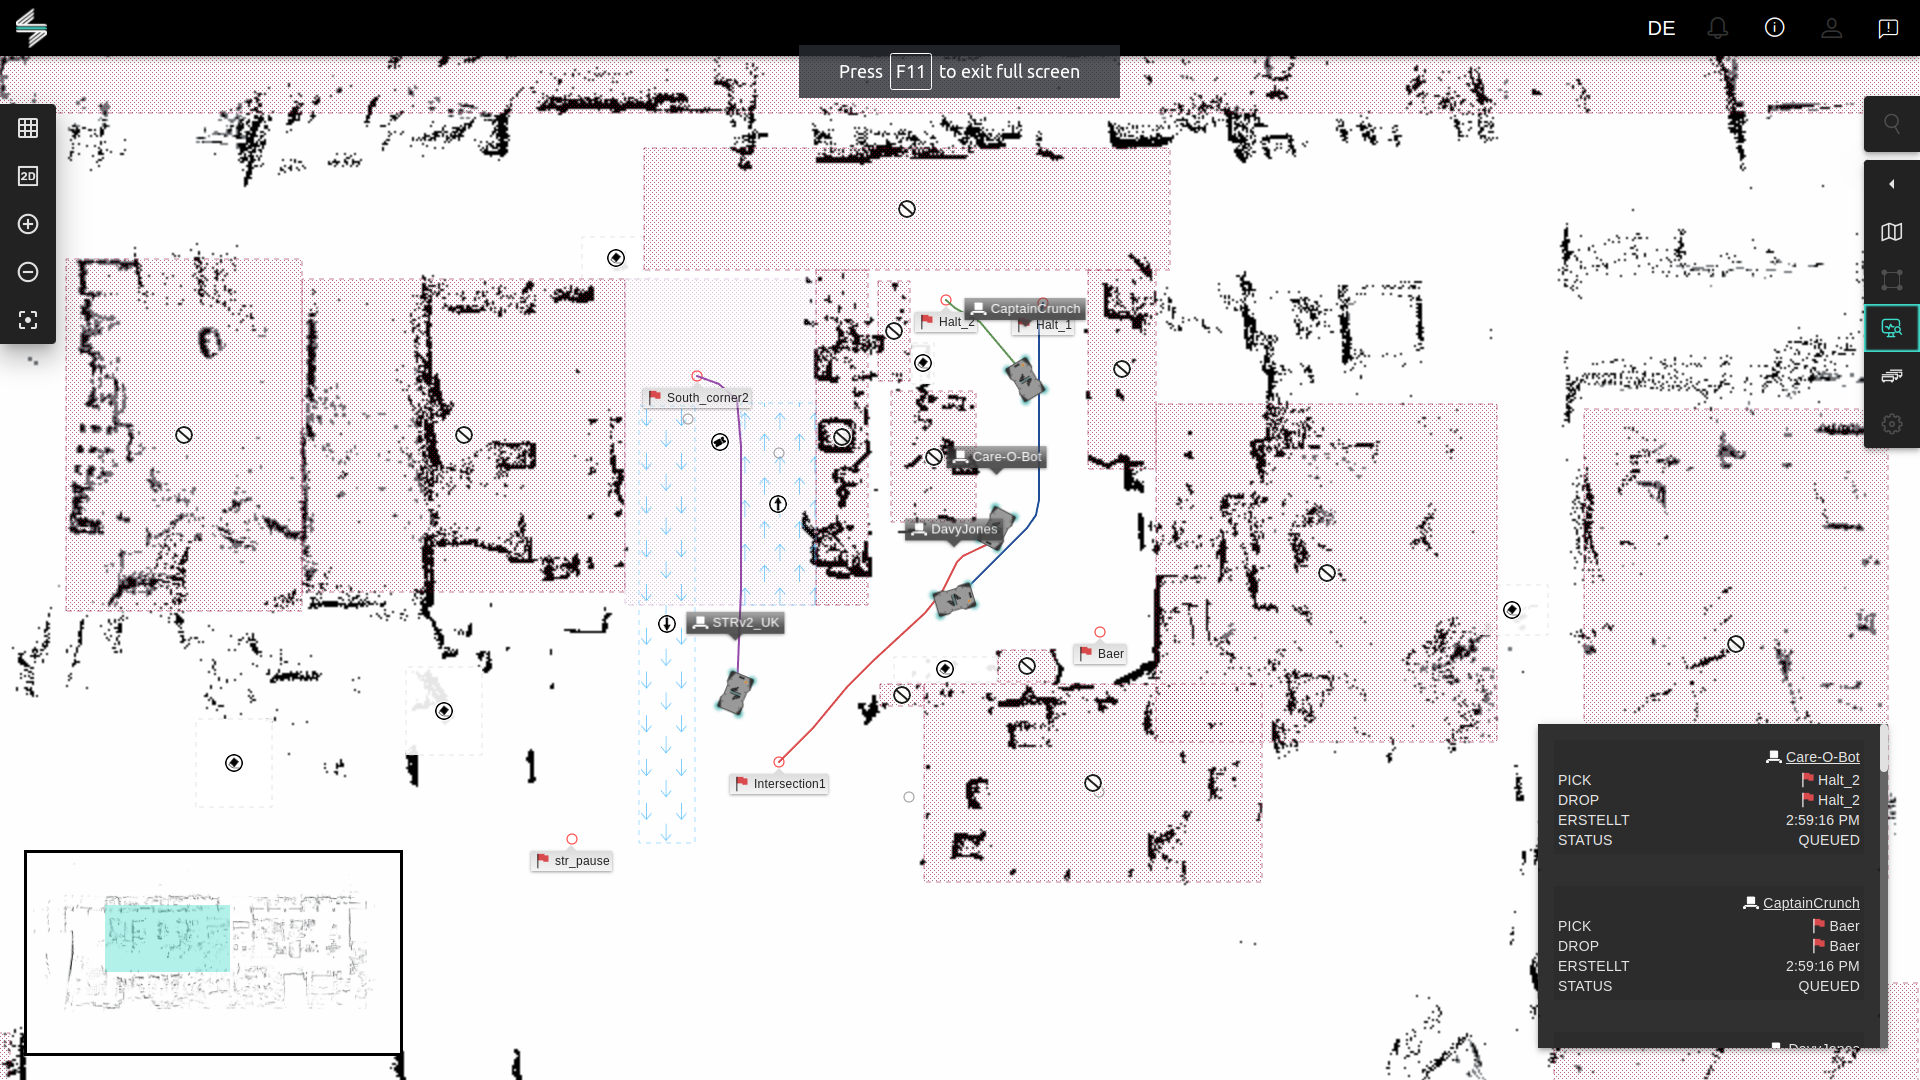
\includegraphics[height=10cm,width=\linewidth]{images/ui_ux.png}
		\caption{Frontend look of Fleet management product of NODE}
	\end{center}
\end{figure}

\section{About robots}
As mentioned NODE solutions are Industrial proof and they are tested for factory environment. This testing will be done on the robots that are available. Before every product release to the customers the release will be tested thoroughly with the available robot. These robots are also used to test any research or new ideas. Here is some of list of robots and their description.

	

\begin{wrapfigure}{r}{0.5\textwidth}
	\centering
	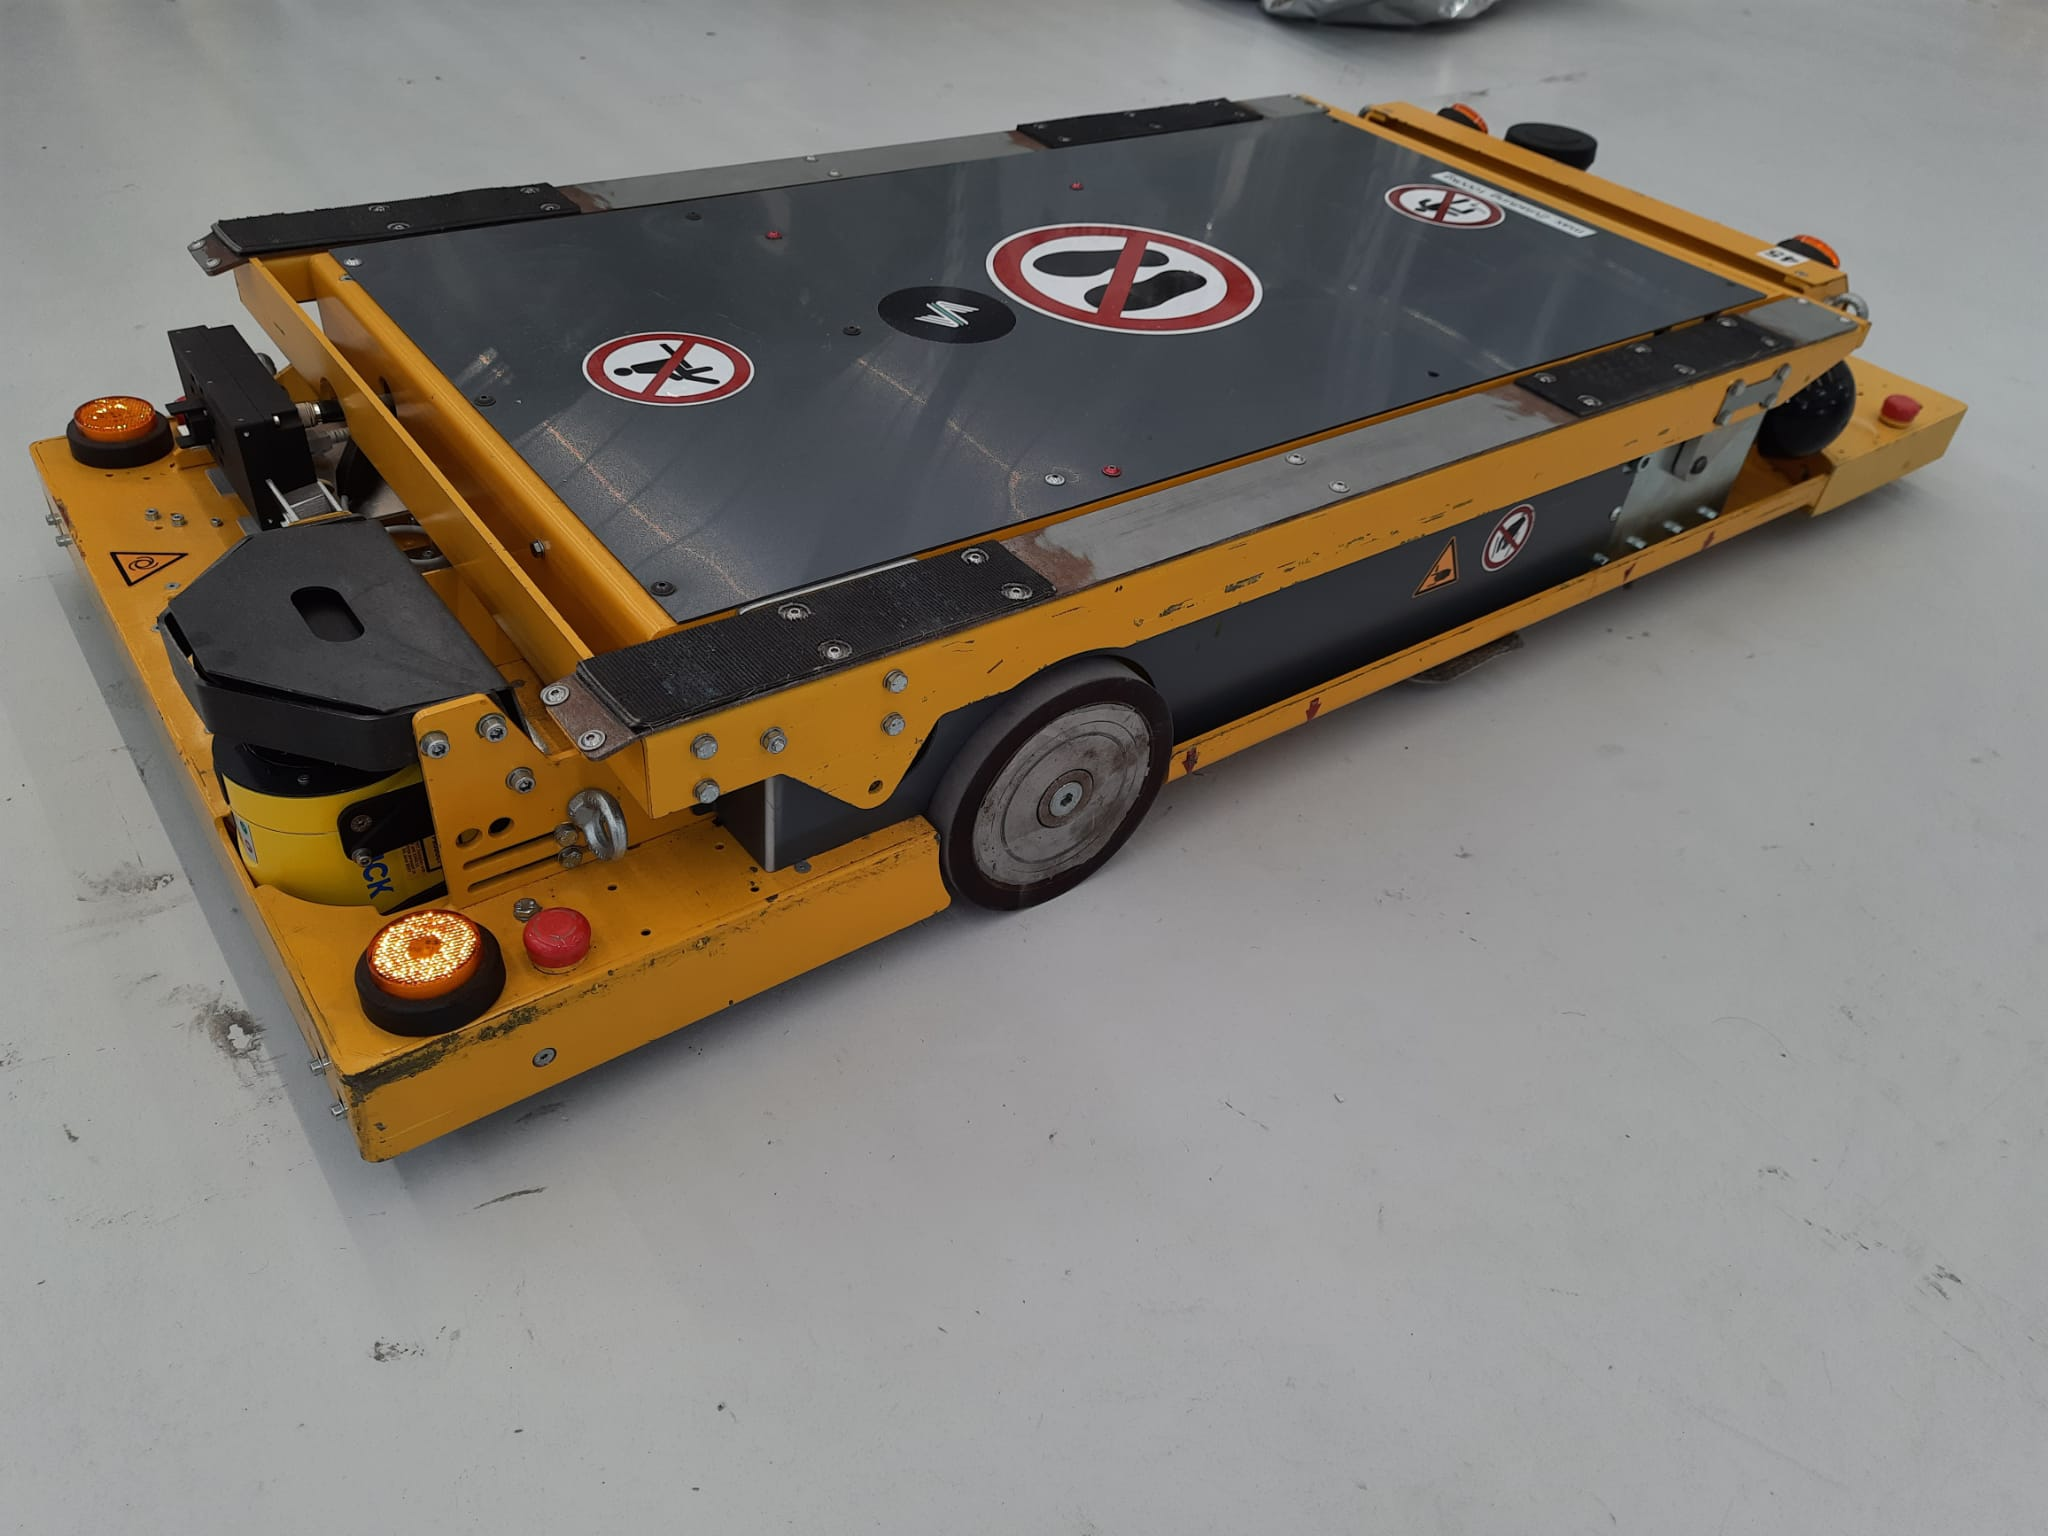
\includegraphics[width=2cm,height=2cm]{images/str.jpeg}
	\caption{STR robot}
\end{wrapfigure}
\subsection{BMW-STR:}
STR are mainly \hspace{2cm}used for the\hspace{2cm} production house in BMW warehouse. This is mainly used \hspace{2cm}to test the releases for the\hspace{2cm} BMW. This robot can lift tons of weight. 

Apart from the str we can also find two different series of Mobile-industrial-robots(MIR)


\begin{wrapfigure}{l}{0.5\textwidth} 
	\centering
	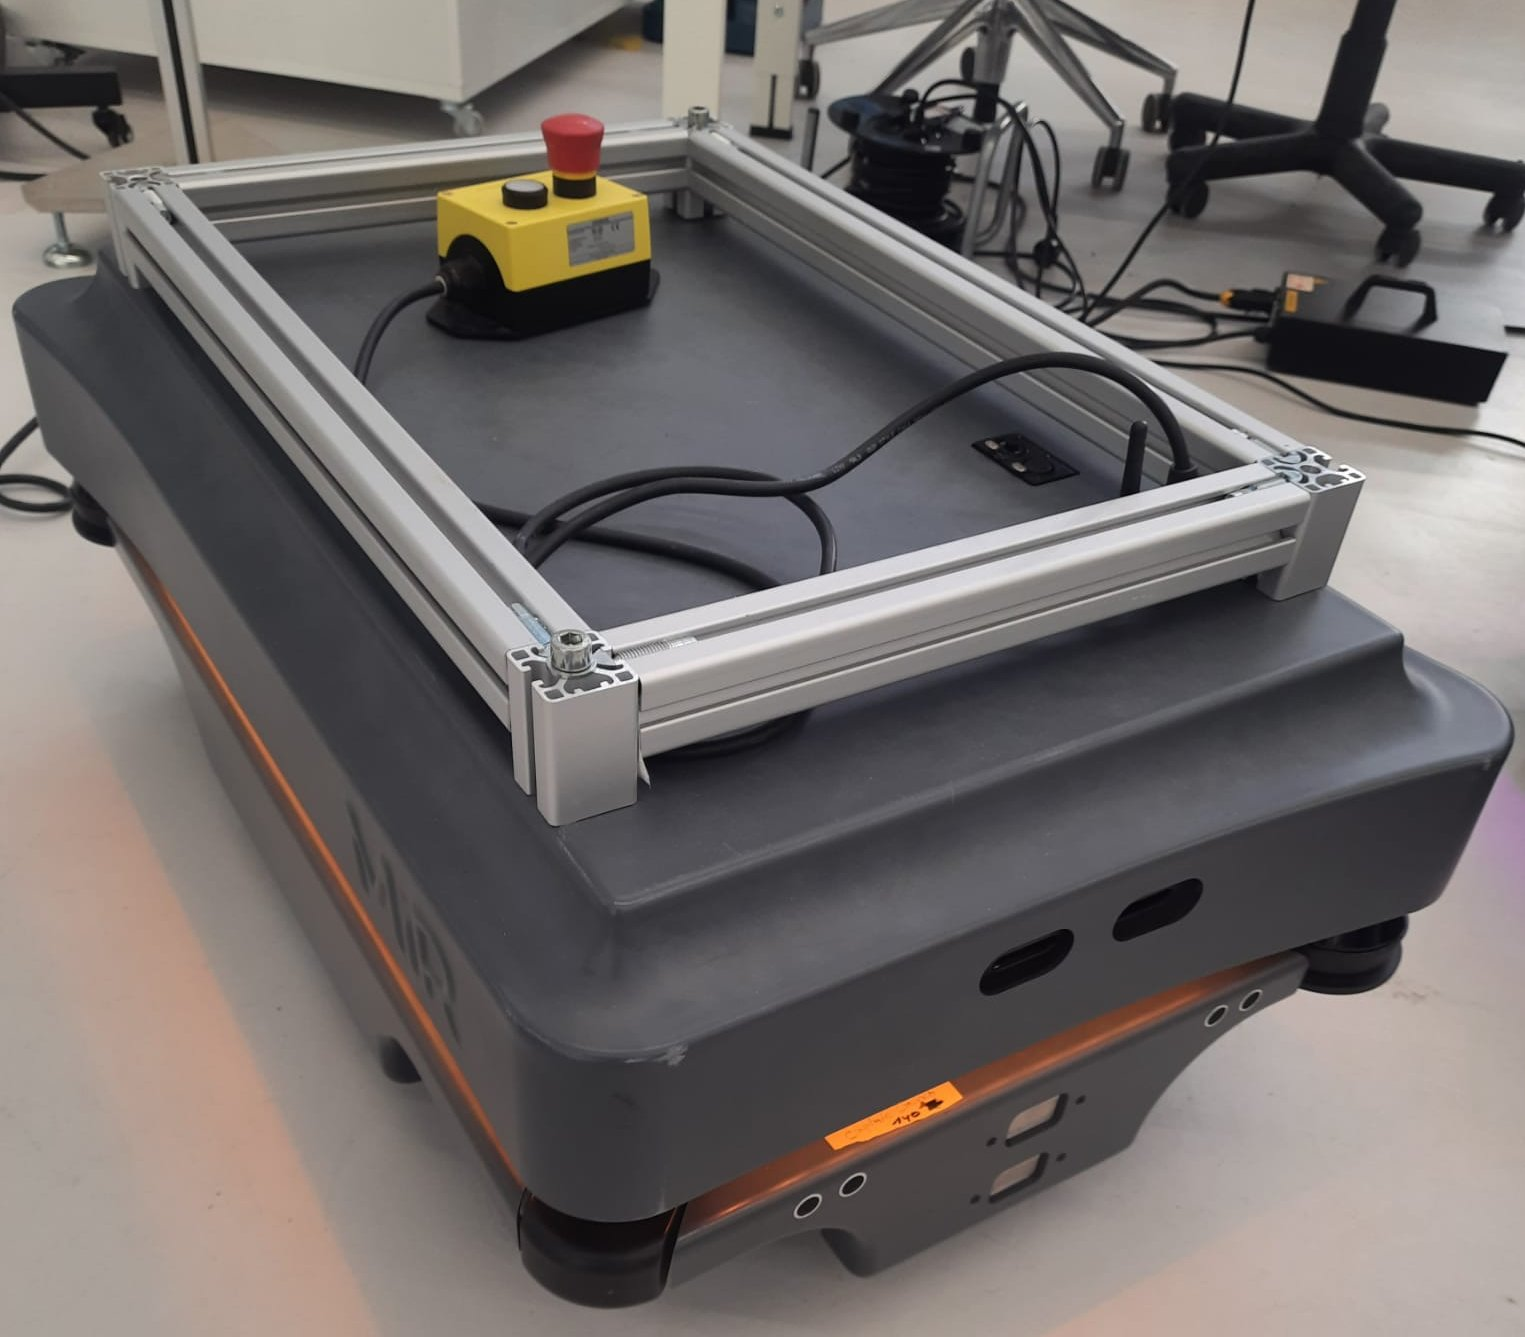
\includegraphics[width=2.5cm,height=2.5cm]{images/mir1.jpeg}
	\caption{mir100 robot}
\end{wrapfigure}
\subsection{MIR100:}
MiR which is known as Mobile industrial robots. This has the maximum speed of 1.5m/s, which can carry up to 100 kg of load. This robot is most suitable for indoor operations. This robot has four ultrasound sensors, two SICK safety laser scanners(front and rear).
	

\begin{wrapfigure}{r}{0.5\textwidth}
	\centering		
	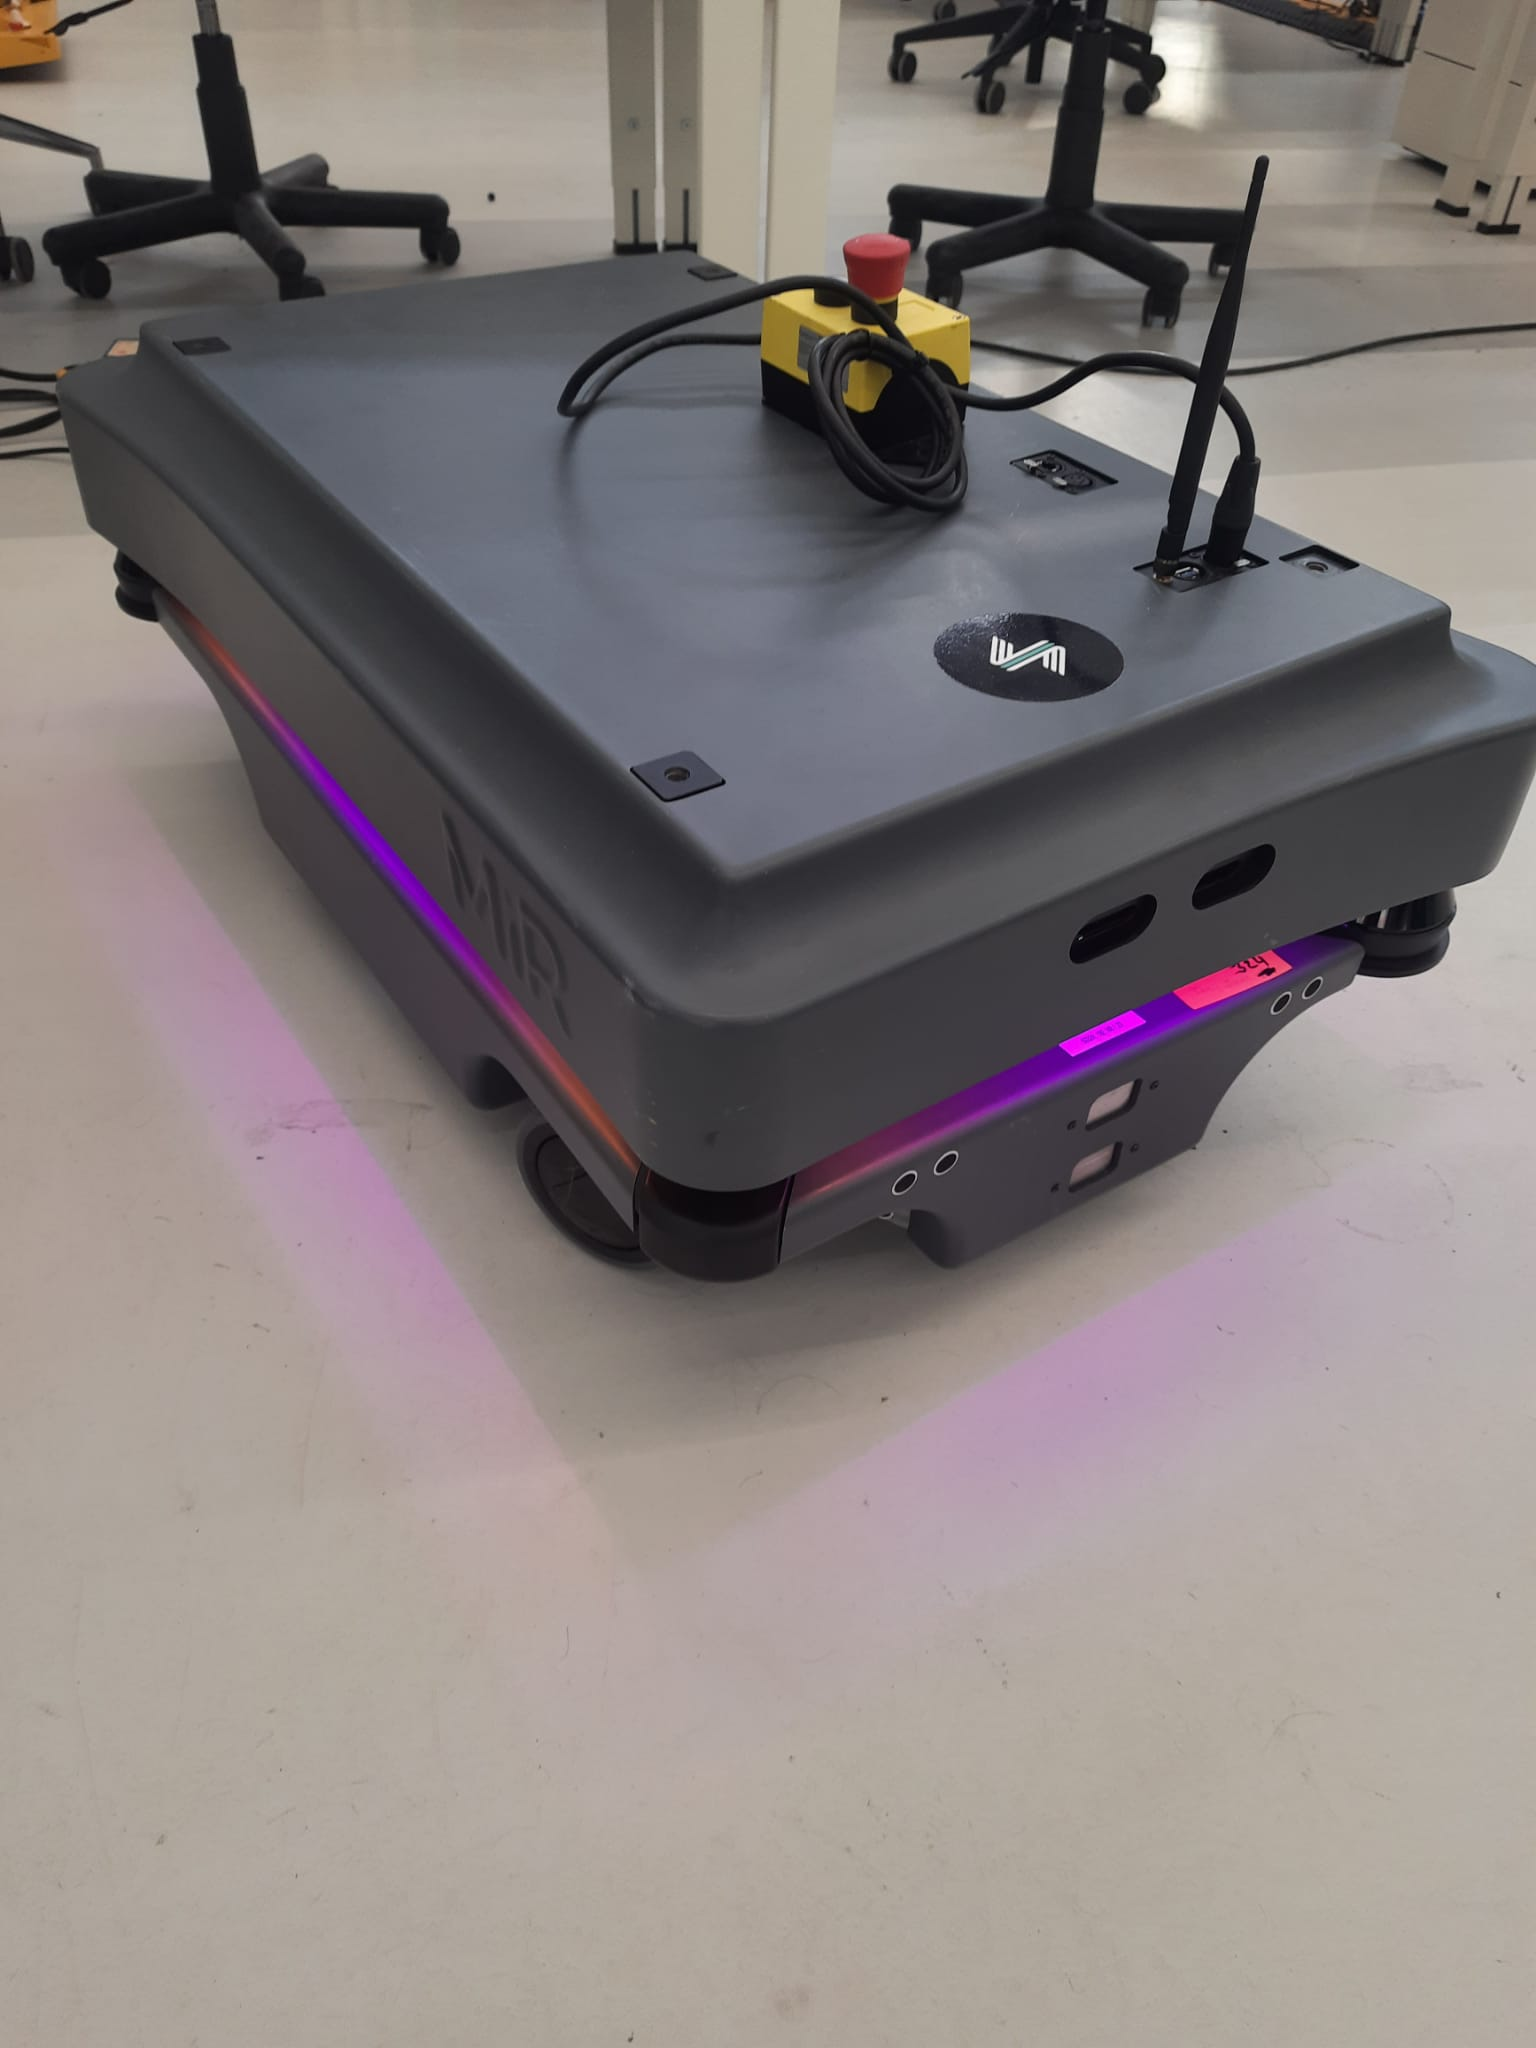
\includegraphics[width=2.5cm,height=2.5cm]{images/mir2.jpeg}
	\caption{mir200 robot}
\end{wrapfigure}
\subsection{MIR200:}	
This robot is a slightly updated version of MIR100. This has the maximum speed of 2.0ms, Payload of 250 kg. This has also feature called over-speed avoidance which prevents the robot from driving faster than predefined safety limit. Safety sensors wise it has same configuration as MIR100.


\begin{wrapfigure}{l}{0.5\textwidth} %this figure will be at the right
	\centering
	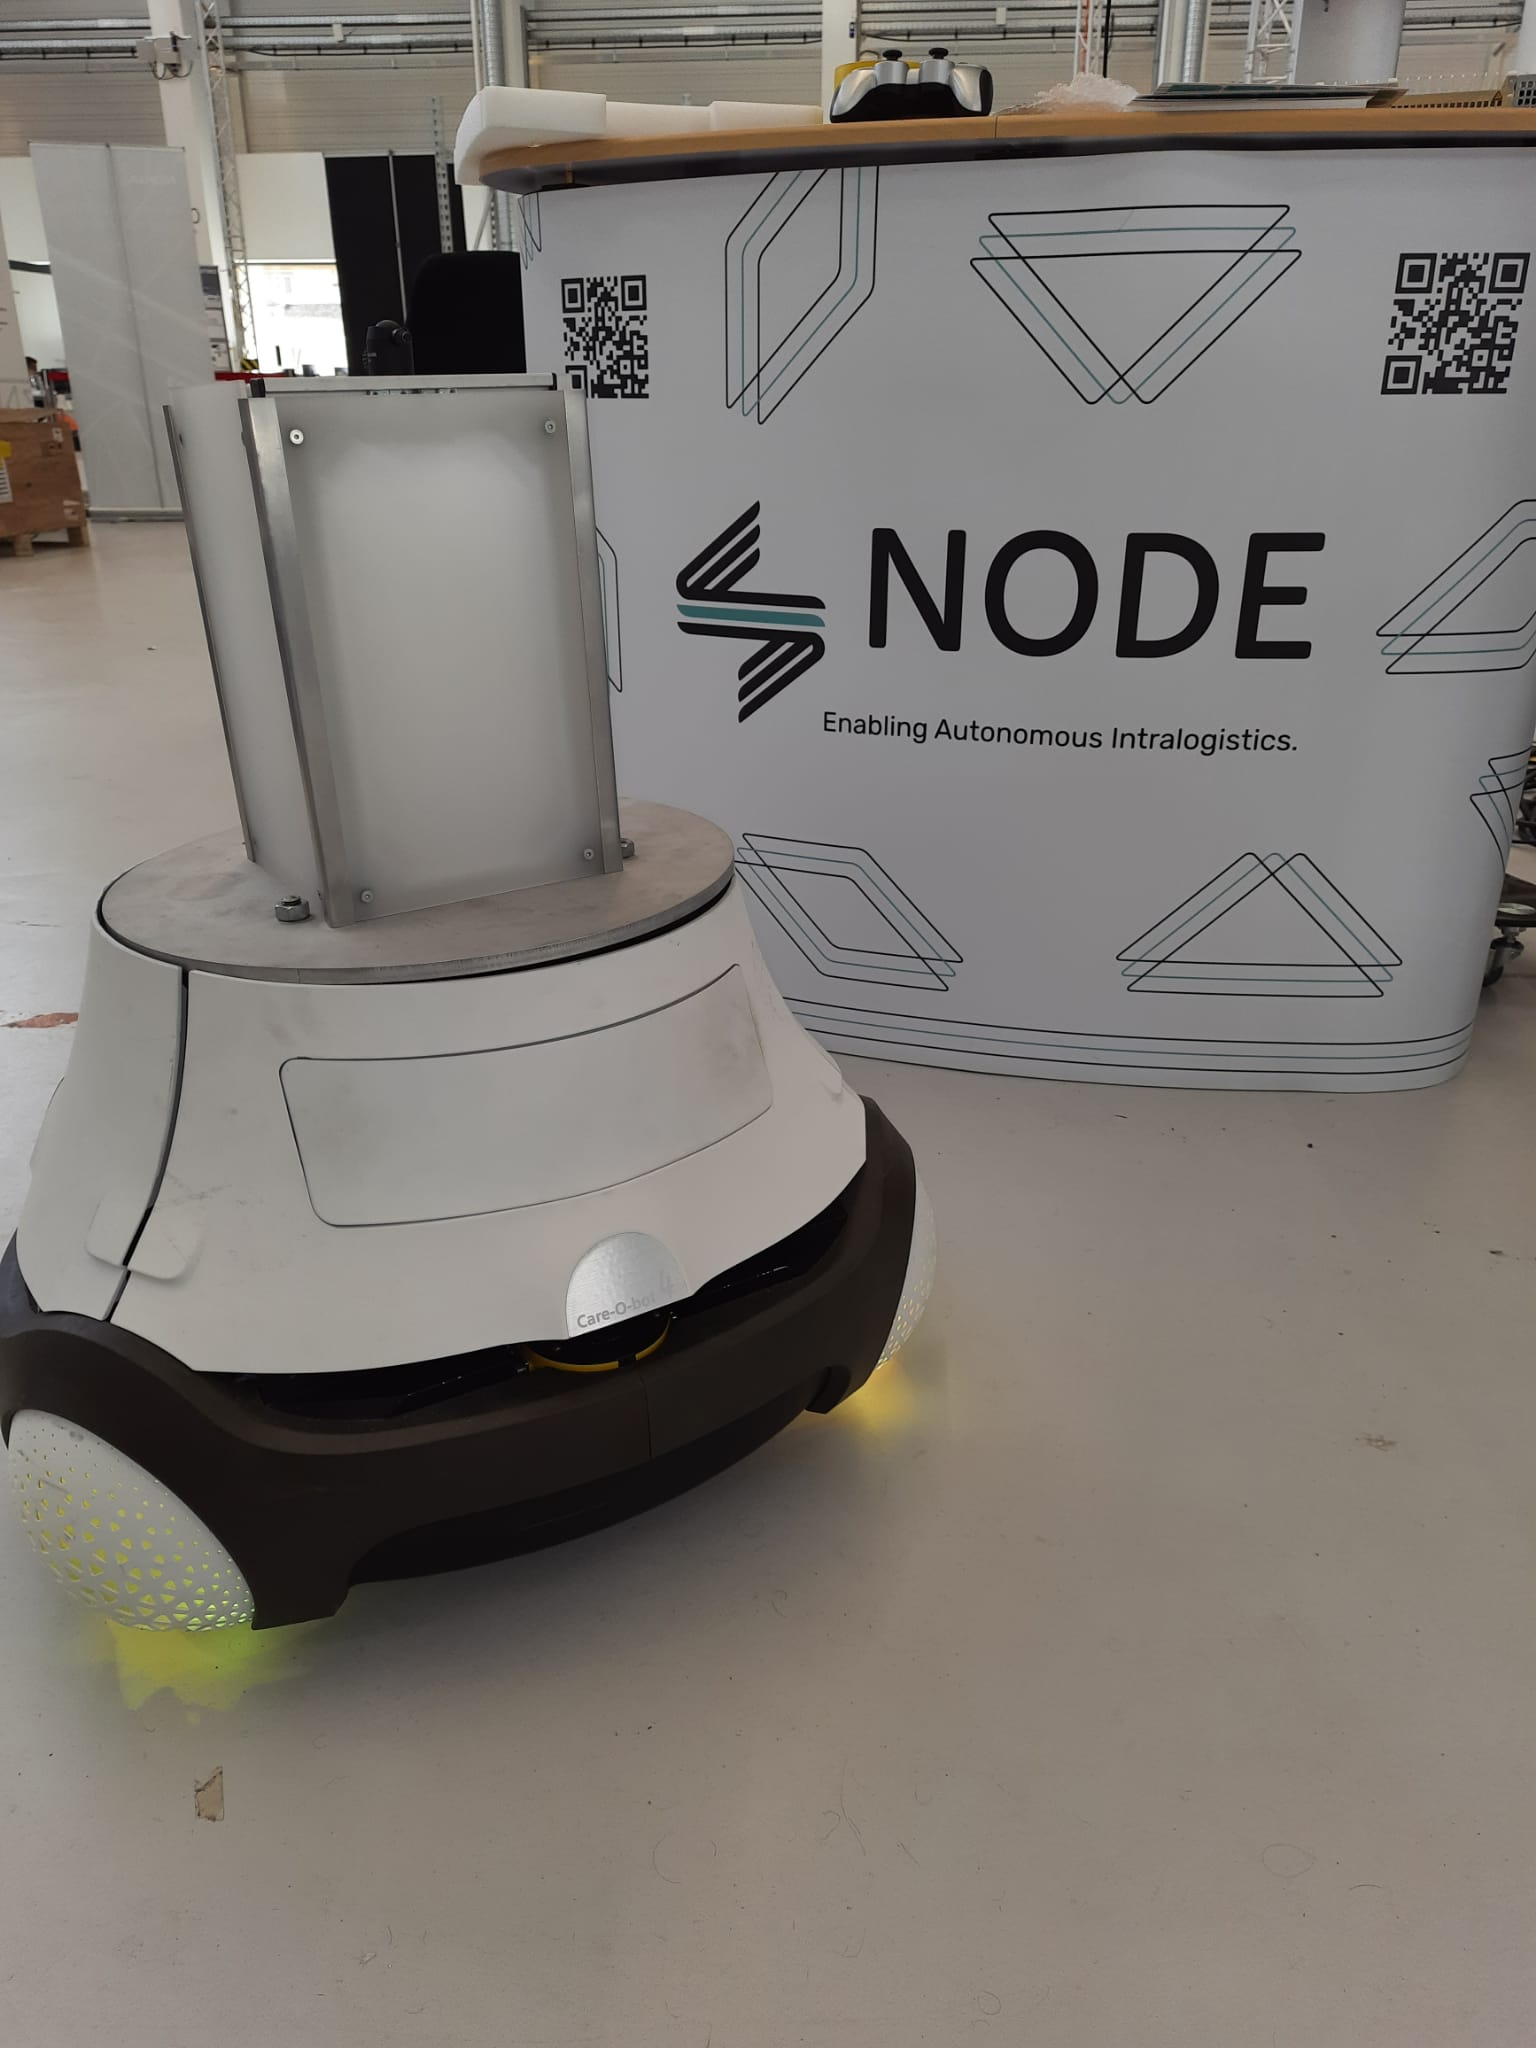
\includegraphics[width=2.5cm,height=2.5cm]{images/cob.jpeg}
	\caption{Care-o-bot}
\end{wrapfigure}
\subsection{Care-O-Bot:}
Care-O-bot is the product vision of a mobile robot assistant to actively support people in the home environment. This robot is omni-directional robot with three wheels. Since the NODE robotics only focusses on the research and development regarding the navigation and fleet, therefore only the lower body of cob is present.
	

With the above robots the operational setup will be done to give some operational demos to some of the companies. This will also be used for research and development.

\begin{figure}[h]
	\begin{center}
		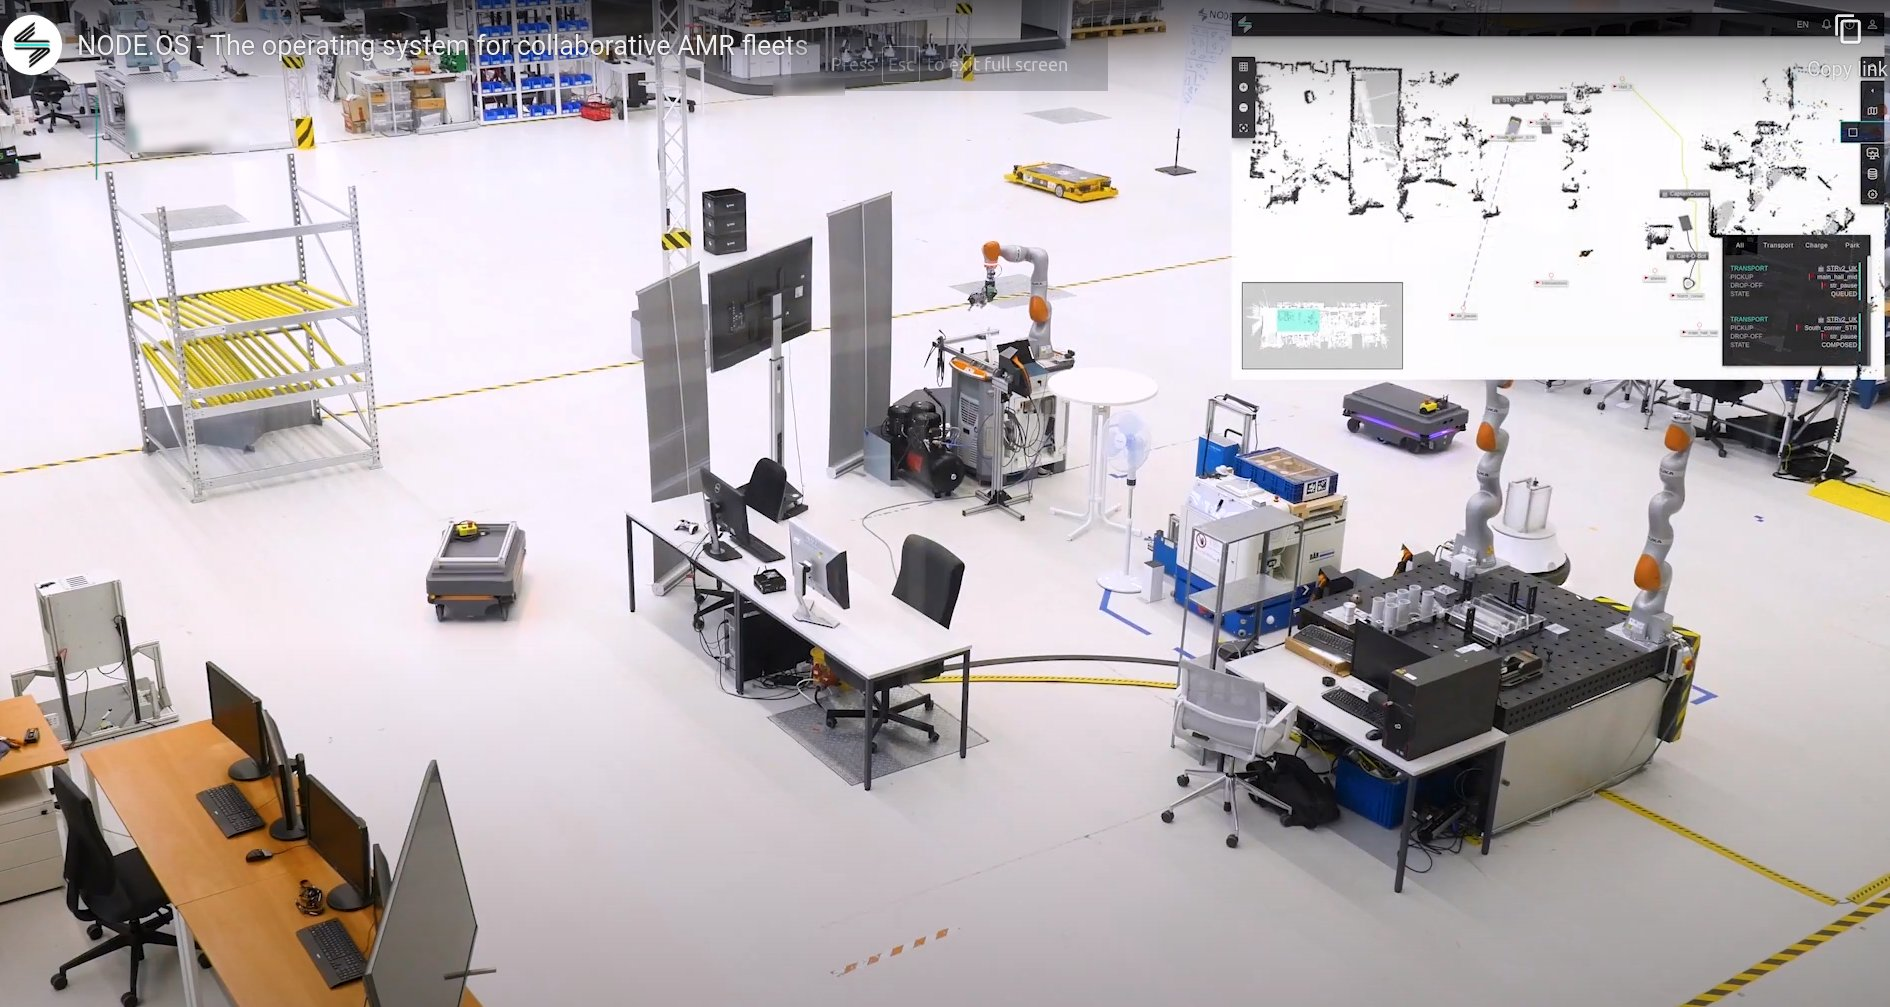
\includegraphics[height=10cm,width=\linewidth]{images/operation.jpg}
		\caption{Workspace of NODE robotics}
	\end{center}
\end{figure}

\pagebreak
\section{Problem statement and research objectives}
\subsection{Problem statement}
As discussed before I worked on a project of developing a UI for rosbag analysis. This was basically part of on-going BMW project. There was a requirement to develop a User-interface which basically analyze the given recorded rosbag. I was given opportunity to support on the backend side of this project. Basically the frontend part like visualizing the robots is basically done by UI-fronend team. We on the backend side should make sure that ROS part works along the frontend. Basic requirements were to play the bag just like playing the video. This included speeding the ROSBAG, stepping to the particular location, loading of rosbag to the cloud, stopping of rosbag. All this has to be done using rosservice call. 

\subsection{Desired outcome}
I was involed in the research of suitable python libraries that can be used to manipulate the rosbag. In this project we must be able to call the rosservice and rostopics using web-sockets. Therefore the communication protocol between the frontend and backend should be done via web-sockets. Also we must use the rosbridge for the communication. 
\subsection{Organization of report}
The report is organized as follows. Chapter 2 will give a brief background of the technical topics that is required to understand this report. This also explains about used during entire internship. Chapter 3 explains about the concept implemented during the internship. This explains why particular concept is chosen to implement the project. Next in Chapter 4 explains the final result of the project. Chapter 5 deals with the various methods that is used to verify and validate the results. Finally chapter 6 gives the final conclusion and future scope.
